\section{Notas de aulas}

As aulas iniciais de Cálculo 3 foram dedicadas ao estudo de funções vetoriais e
às principais operações de cálculo aplicadas a essas funções. Nesta seção, são
reunidas as definições, teoremas, propriedades e problemas apresentados durante
as aulas, abrangendo conceitos como limite e continuidade de funções vetoriais,
derivadas, retas tangentes, derivadas de produtos escalares e vetoriais,
integrais e antiderivadas de funções vetoriais.

\section*{Funções Vetoriais}

\definition{Função Vetorial}{
  Uma \textbf{função vetorial} é uma função cujo domínio é um conjunto de
  números reais e cujos valores são vetores. No espaço tridimensional, uma
  função vetorial pode ser escrita na forma

	\[
		\mathbf{r}(t)
		=
		x(t)\mathbf{i}
		+y(t)\mathbf{j}
		+z(t)\mathbf{k},
	\]

	onde $x(t)$, $y(t)$ e $z(t)$ são funções reais da variável $t$.

	Equivalentemente,

	\[
		\mathbf{r}(t)
		=
		\left\langle
		x(t),y(t),z(t)
		\right\rangle.
	\]
}

\definition{Limite de uma Função Vetorial}{
  Seja $\mathbf{r}(t)$ uma função vetorial definida em cada $t$ de algum
  intervalo aberto contendo $a$, exceto que $\mathbf{r}(t)$ não precisa estar
  definida em $a$. Dizemos que

	\[
		\lim_{t\to a}\mathbf{r}(t)=\mathbf{L}
	\]

	se, e somente se,

	\[
		\lim_{t\to a}
		\left\|\mathbf{r}(t)-\mathbf{L}\right\|=0.
	\]

	Se

	\[
		\mathbf{r}(t)
		=
		\left\langle
		x(t),y(t),z(t)
		\right\rangle,
	\]

	então o limite pode ser calculado componente a componente:

	\[
		\lim_{t\to a}\mathbf{r}(t)
		=
		\left\langle
		\lim_{t\to a}x(t),
		\lim_{t\to a}y(t),
		\lim_{t\to a}z(t)
		\right\rangle,
	\]

	desde que os limites das componentes existam.
}

\question{
	Seja
	\[
		\mathbf{r}(t)
		=
		t^2\mathbf{i}
		+e^t\mathbf{j}
		-2\cos(\pi t)\mathbf{k}.
	\]
	Calcule
	\[
		\lim_{t\to0}\mathbf{r}(t).
	\]
}

\answer{
	Calculando o limite componente a componente,

	\[
		\begin{aligned}
		\lim_{t\to0}t^2 &= 0,\\
		\lim_{t\to0}e^t &= 1,\\
		\lim_{t\to0}-2\cos(\pi t) &= -2.
		\end{aligned}
	\]

	Portanto,

	\[
		\boxed{
		\lim_{t\to0}\mathbf{r}(t)
		=
		0\mathbf{i}+\mathbf{j}-2\mathbf{k}
		}
	\]

	ou, equivalentemente,

	\[
		\boxed{\left\langle 0,1,-2\right\rangle}.
	\]
}

\definition{Derivada de uma Função Vetorial}{
	Seja $\mathbf{r}(t)$ uma função vetorial. A \textbf{derivada de
	$\mathbf{r}$ em relação a $t$} é a função vetorial $\mathbf{r}'$ definida por

	\[
		\mathbf{r}'(t)
		=
		\lim_{h\to0}
		\frac{\mathbf{r}(t+h)-\mathbf{r}(t)}{h},
	\]

	quando esse limite existe.

	O domínio de $\mathbf{r}'$ consiste em todos os valores de $t$ do domínio
	de $\mathbf{r}(t)$ para os quais o limite acima existe.
}

\definition{Derivada por Componentes}{
	Seja

	\[
		\mathbf{r}(t)
		=
		\left\langle
		x(t),y(t),z(t)
		\right\rangle.
	\]

	A função vetorial $\mathbf{r}(t)$ é diferenciável em $t$ se, e somente se,
	cada uma de suas funções componentes for diferenciável em $t$. Nesse caso,

	\[
		\mathbf{r}'(t)
		=
		\left\langle
		x'(t),y'(t),z'(t)
		\right\rangle.
	\]

	Assim, a derivação de uma função vetorial pode ser realizada
	componente a componente.
}

\question{
	Seja
	\[
		\mathbf{r}(t)
		=
		t^2\mathbf{i}
		+e^t\mathbf{j}
		-2\cos(\pi t)\mathbf{k}.
	\]
	Determine $\mathbf{r}'(t)$.
}

\answer{
	Derivando a função vetorial componente a componente, temos

	\[
		\mathbf{r}'(t)
		=
		\frac{d}{dt}(t^2)\mathbf{i}
		+\frac{d}{dt}(e^t)\mathbf{j}
		-\frac{d}{dt}\left(2\cos(\pi t)\right)\mathbf{k}.
	\]

	Como

	\[
		\frac{d}{dt}(t^2)=2t,
		\qquad
		\frac{d}{dt}(e^t)=e^t,
	\]

	e, pela regra da cadeia,

	\[
		\frac{d}{dt}\left[-2\cos(\pi t)\right]
		=
		2\pi\sin(\pi t),
	\]

	obtemos

	\[
		\boxed{
		\mathbf{r}'(t)
		=
		2t\mathbf{i}
		+e^t\mathbf{j}
		+2\pi\sin(\pi t)\mathbf{k}
		}.
	\]
}

\definition{Regras de Derivação de Funções Vetoriais}{
	Sejam $\mathbf{r}(t)$, $\mathbf{r}_1(t)$ e $\mathbf{r}_2(t)$ funções
	vetoriais, $f(t)$ uma função real, $k$ um escalar e $\mathbf{c}$ um vetor
	constante. Quando as derivadas existem, valem as seguintes regras:

	\[
		\frac{d}{dt}
		\left[
			\mathbf{r}_1(t)+\mathbf{r}_2(t)
		\right]
		=
		\mathbf{r}_1'(t)+\mathbf{r}_2'(t),
	\]

	\[
		\frac{d}{dt}
		\left[
			k\mathbf{r}(t)
		\right]
		=
		k\mathbf{r}'(t),
	\]

	\[
		\frac{d}{dt}
		\left[
			f(t)\mathbf{r}(t)
		\right]
		=
		f'(t)\mathbf{r}(t)
		+
		f(t)\mathbf{r}'(t),
	\]

	\[
		\frac{d}{dt}
		\left[
			\mathbf{r}(t)\cdot\mathbf{c}
		\right]
		=
		\mathbf{r}'(t)\cdot\mathbf{c}.
	\]
}

\definition{Vetor Tangente}{
	Seja $P$ um ponto no gráfico de uma função vetorial $\mathbf{r}(t)$,
	correspondente a $t=t_0$. Se $\mathbf{r}'(t_0)$ existir e
	$\mathbf{r}'(t_0)\neq\mathbf{0}$, então $\mathbf{r}'(t_0)$ é denominado
	\textbf{vetor tangente} ao gráfico de $\mathbf{r}(t)$ em
	$\mathbf{r}(t_0)$.

	A reta que passa pelo ponto $P$ e é paralela ao vetor tangente é denominada
	\textbf{reta tangente} ao gráfico de $\mathbf{r}(t)$ em $t=t_0$.

	Se

	\[
		\mathbf{r}_0=\mathbf{r}(t_0)
		\qquad\text{e}\qquad
		\mathbf{v}_0=\mathbf{r}'(t_0),
	\]

	então a reta tangente é dada por

	\[
		\mathbf{r}
		=
		\mathbf{r}_0+s\mathbf{v}_0,
	\]

	onde $s\in\mathbb{R}$.
}

\question{
	Obtenha equações paramétricas da reta tangente à hélice circular
	\[
	\begin{cases}
		x &= \cos t,\\
		y &= \sin t,\\
		z &= t,
	\end{cases}
	\]
  no ponto correspondente a $t=t_0$, e use esse resultado para obter equações
  paramétricas da reta tangente no ponto em que $t=\frac{\pi}{2}$.
}

\answer{
	A hélice circular pode ser representada pela função vetorial

	\[
		\mathbf{r}(t)
		=
		\left\langle
		\cos t,\sin t,t
		\right\rangle.
	\]

	O vetor tangente é obtido derivando $\mathbf{r}(t)$:

	\[
		\mathbf{r}'(t)
		=
		\left\langle
		-\sin t,\cos t,1
		\right\rangle.
	\]

	No ponto correspondente a $t=t_0$, temos

	\[
		\mathbf{r}(t_0)
		=
		\left\langle
		\cos t_0,\sin t_0,t_0
		\right\rangle
	\]

	e o vetor tangente

	\[
		\mathbf{r}'(t_0)
		=
		\left\langle
		-\sin t_0,\cos t_0,1
		\right\rangle.
	\]

	Portanto, as equações paramétricas da reta tangente são

	\[
		\boxed{
		\begin{cases}
			x=\cos t_0-s\sin t_0,\\
			y=\sin t_0+s\cos t_0,\\
			z=t_0+s,
		\end{cases}
		\qquad s\in\mathbb{R}.
		}
	\]

  Para $t_0=\frac{\pi}{2}$,

	\[
	\cos\frac{\pi}{2}=0,
	\qquad
	\sin\frac{\pi}{2}=1.
	\]

	Assim, o ponto da hélice é

	\[
	\mathbf{r}\left(\frac{\pi}{2}\right)
	=
	\left\langle
	0,1,\frac{\pi}{2}
	\right\rangle
	\]

	e o vetor tangente é

	\[
	\mathbf{r}'\left(\frac{\pi}{2}\right)
	=
	\langle -1,0,1\rangle.
	\]

	Logo, as equações paramétricas da reta tangente são

	\[
	\boxed{
	\begin{cases}
		x=-s,\\
		y=1,\\
		z=\dfrac{\pi}{2}+s,
	\end{cases}
	\qquad s\in\mathbb{R}.
	}
	\]
}

\definition{Derivada de um Produto Escalar}{
	Sejam $\mathbf{r}_1(t)$ e $\mathbf{r}_2(t)$ funções vetoriais
	diferenciáveis. Então,

	\[
		\frac{d}{dt}
		\left[
			\mathbf{r}_1(t)\cdot\mathbf{r}_2(t)
		\right]
		=
		\mathbf{r}_1'(t)\cdot\mathbf{r}_2(t)
		+
		\mathbf{r}_1(t)\cdot\mathbf{r}_2'(t).
	\]
}

\definition{Derivada de um Produto Vetorial}{
	Sejam $\mathbf{r}_1(t)$ e $\mathbf{r}_2(t)$ funções vetoriais
	diferenciáveis. Então,

	\[
		\frac{d}{dt}
		\left[
			\mathbf{r}_1(t)\times\mathbf{r}_2(t)
		\right]
		=
		\mathbf{r}_1'(t)\times\mathbf{r}_2(t)
		+
		\mathbf{r}_1(t)\times\mathbf{r}_2'(t).
	\]
}

\definition{Integral de uma Função Vetorial}{
	Seja $\mathbf{r}(t)$ uma função vetorial contínua no intervalo
	$[a,b]$, escrita como

	\[
		\mathbf{r}(t)
		=
		\left\langle
		x(t),y(t),z(t)
		\right\rangle.
	\]

	A integral definida de $\mathbf{r}(t)$ em $[a,b]$ é calculada
	componente a componente:

	\[
		\int_a^b\mathbf{r}(t)\,dt
		=
		\left\langle
		\int_a^b x(t)\,dt,
		\int_a^b y(t)\,dt,
		\int_a^b z(t)\,dt
		\right\rangle.
	\]
}

\question{
	Calcule
	\[
		\int_0^1\mathbf{r}(t)\,dt,
	\]
	onde
	\[
		\mathbf{r}(t)
		=
		t^2\mathbf{i}
		+e^t\mathbf{j}
		-2\cos(\pi t)\mathbf{k}.
	\]
}

\answer{
	A integral de uma função vetorial pode ser calculada componente a
	componente. Portanto,

	\[
	\begin{aligned}
		\int_0^1\mathbf{r}(t)\,dt
		&=
		\int_0^1
		\left(
			t^2\mathbf{i}
			+e^t\mathbf{j}
			-2\cos(\pi t)\mathbf{k}
		\right)dt\\
		&=
		\left(\int_0^1t^2\,dt\right)\mathbf{i}
		+
		\left(\int_0^1e^t\,dt\right)\mathbf{j}
		-
		2\left(\int_0^1\cos(\pi t)\,dt\right)\mathbf{k}.
	\end{aligned}
	\]

	Calculando cada componente,

	\[
		\int_0^1t^2\,dt
		=
		\left.\frac{t^3}{3}\right|_0^1
		=
		\frac{1}{3},
	\]

	\[
		\int_0^1e^t\,dt
		=
		\left.e^t\right|_0^1
		=
		e-1,
	\]

	e

	\[
		-2\int_0^1\cos(\pi t)\,dt
		=
		-2\left.\frac{\sin(\pi t)}{\pi}\right|_0^1
		=
		0.
	\]

	Logo,

	\[
		\boxed{
		\int_0^1\mathbf{r}(t)\,dt
		=
		\frac{1}{3}\mathbf{i}
		+(e-1)\mathbf{j}
		}.
	\]
}

\definition{Regras de Integração de Funções Vetoriais}{
	Sejam $\mathbf{r}(t)$, $\mathbf{r}_1(t)$ e $\mathbf{r}_2(t)$ funções
	vetoriais contínuas no intervalo $[a,b]$ e seja $k$ um escalar. Então,

	\[
		\int_a^b
		\left[
			\mathbf{r}_1(t)+\mathbf{r}_2(t)
		\right]dt
		=
		\int_a^b\mathbf{r}_1(t)\,dt
		+
		\int_a^b\mathbf{r}_2(t)\,dt,
	\]

	\[
		\int_a^b
		k\mathbf{r}(t)\,dt
		=
		k\int_a^b\mathbf{r}(t)\,dt.
	\]
}

\definition{Antiderivada de uma Função Vetorial}{
	Uma função vetorial $\mathbf{R}(t)$ é denominada \textbf{antiderivada}
	de uma função vetorial $\mathbf{r}(t)$ em um intervalo se

	\[
		\mathbf{R}'(t)=\mathbf{r}(t).
	\]

	Usando a notação de integral, escrevemos

	\[
		\int\mathbf{r}(t)\,dt
		=
		\mathbf{R}(t)+\mathbf{C},
	\]

	onde $\mathbf{C}$ representa um vetor constante arbitrário.

	Se

	\[
		\mathbf{r}(t)
		=
		\left\langle
		x(t),y(t),z(t)
		\right\rangle,
	\]

	então

	\[
		\int\mathbf{r}(t)\,dt
		=
		\left\langle
		\int x(t)\,dt,
		\int y(t)\,dt,
		\int z(t)\,dt
		\right\rangle
		+\mathbf{C}.
  \]
}

\question{
	Determine uma antiderivada da função vetorial
	\[
		\mathbf{r}(t)
		=
		t^2\mathbf{i}
		+e^t\mathbf{j}
		-2\cos(\pi t)\mathbf{k}.
	\]
}

\answer{
	Uma antiderivada de uma função vetorial é obtida integrando cada uma de
	suas componentes. Assim,

	\[
	\begin{aligned}
		\int \mathbf{r}(t)\,dt
		&=
		\int
		\left(
			t^2\mathbf{i}
			+e^t\mathbf{j}
			-2\cos(\pi t)\mathbf{k}
		\right)dt\\
		&=
		\left(\int t^2\,dt\right)\mathbf{i}
		+
		\left(\int e^t\,dt\right)\mathbf{j}
		-
		2\left(\int\cos(\pi t)\,dt\right)\mathbf{k}.
	\end{aligned}
	\]

	Calculando cada integral,

	\[
		\int t^2\,dt=\frac{t^3}{3},
		\qquad
		\int e^t\,dt=e^t,
	\]

	e, pela regra da cadeia,

	\[
		-2\int\cos(\pi t)\,dt
		=
		-\frac{2}{\pi}\sin(\pi t).
	\]

	Portanto, uma antiderivada é

	\[
		\boxed{
		\mathbf{R}(t)
		=
		\frac{t^3}{3}\mathbf{i}
		+e^t\mathbf{j}
		-\frac{2}{\pi}\sin(\pi t)\mathbf{k}
		+\mathbf{C}
		},
	\]

	onde $\mathbf{C}$ é um vetor constante arbitrário.
}

\section*{Comprimento do Arco}

\definition{Comprimento de Arco de uma Curva Paramétrica}{
	Seja
	\[
		x=x(t),\qquad y=y(t),\qquad a\leq t\leq b,
	\]
	uma curva paramétrica no plano. Seu comprimento de arco é dado por

	\[
		L
		=
		\int_a^b
		\sqrt{
			[x'(t)]^2+[y'(t)]^2
		}\,dt.
	\]

	De forma análoga, se
	\[
		x=x(t),\qquad
		y=y(t),\qquad
		z=z(t),
		\qquad a\leq t\leq b,
	\]
	é uma curva paramétrica no espaço tridimensional, então seu comprimento
	de arco é

	\[
		L
		=
		\int_a^b
		\sqrt{
			[x'(t)]^2
			+[y'(t)]^2
			+[z'(t)]^2
		}\,dt.
	\]
}

\definition{Comprimento de Arco do Ponto de Vista Vetorial}{
	Seja $\mathbf{r}(t)$ uma função vetorial lisa que descreve uma curva
	no plano ou no espaço. Para uma curva plana,

	\[
		\mathbf{r}(t)
		=
		\left\langle
		x(t),y(t)
		\right\rangle,
	\]

	enquanto, para uma curva no espaço tridimensional,

	\[
		\mathbf{r}(t)
		=
		\left\langle
		x(t),y(t),z(t)
		\right\rangle.
	\]

	A derivada de $\mathbf{r}(t)$ é, respectivamente,

	\[
		\mathbf{r}'(t)
		=
		\left\langle
		x'(t),y'(t)
		\right\rangle
	\]

	e

	\[
		\mathbf{r}'(t)
		=
		\left\langle
		x'(t),y'(t),z'(t)
		\right\rangle.
	\]

	Portanto, sua norma é

	\[
		\left\|\mathbf{r}'(t)\right\|
		=
		\sqrt{
			[x'(t)]^2+[y'(t)]^2
		}
	\]

	no plano e

	\[
		\left\|\mathbf{r}'(t)\right\|
		=
		\sqrt{
			[x'(t)]^2
			+[y'(t)]^2
			+[z'(t)]^2
		}
	\]

	no espaço.

	Assim, as fórmulas de comprimento de arco podem ser escritas de forma
	unificada em termos da função vetorial $\mathbf{r}(t)$.
}

\definition{Teorema do Comprimento de Arco}{
	Se $C$ for o gráfico no espaço bidimensional ou tridimensional de uma
	função vetorial lisa $\mathbf{r}(t)$, então seu comprimento de arco de
	$t=a$ até $t=b$ é

	\[
		\boxed{
		L
		=
		\int_a^b
		\left\|\mathbf{r}'(t)\right\|\,dt
		}.
	\]

	Essa fórmula é válida tanto para curvas planas quanto para curvas
	tridimensionais.
}

\question{
	Determine o comprimento de arco da curva representada pela função
	vetorial

	\[
		\mathbf{r}(t)
		=
		\left\langle
		x(t),y(t),z(t)
		\right\rangle,
		\qquad a\leq t\leq b.
	\]
}

\answer{
	Para determinar o comprimento de arco, inicialmente calculamos a derivada
	da função vetorial:

	\[
		\mathbf{r}'(t)
		=
		\left\langle
		x'(t),y'(t),z'(t)
		\right\rangle.
	\]

	Em seguida, calculamos sua norma:

	\[
		\left\|\mathbf{r}'(t)\right\|
		=
		\sqrt{
			[x'(t)]^2
			+[y'(t)]^2
			+[z'(t)]^2
		}.
	\]

	Aplicando o Teorema do Comprimento de Arco,

	\[
		L
		=
		\int_a^b
		\left\|\mathbf{r}'(t)\right\|\,dt.
	\]

	Logo,

	\[
		\boxed{
		L
		=
		\int_a^b
		\sqrt{
			[x'(t)]^2
			+[y'(t)]^2
			+[z'(t)]^2
		}\,dt
		}.
	\]
}

\subquestion{
	Por que a fórmula vetorial
	\[
		L=\int_a^b\|\mathbf{r}'(t)\|\,dt
	\]
	é equivalente às fórmulas usuais de comprimento de arco?
}

\answer{
	Se

	\[
		\mathbf{r}(t)
		=
		\left\langle
		x(t),y(t),z(t)
		\right\rangle,
	\]

	então

	\[
		\mathbf{r}'(t)
		=
		\left\langle
		x'(t),y'(t),z'(t)
		\right\rangle.
	\]

	Pela definição da norma de um vetor,

	\[
		\left\|\mathbf{r}'(t)\right\|
		=
		\sqrt{
			[x'(t)]^2
			+[y'(t)]^2
			+[z'(t)]^2
		}.
	\]

	Substituindo essa expressão na fórmula vetorial,

	\[
		L
		=
		\int_a^b
		\left\|\mathbf{r}'(t)\right\|\,dt,
	\]

	obtemos

	\[
		L
		=
		\int_a^b
		\sqrt{
			[x'(t)]^2
			+[y'(t)]^2
			+[z'(t)]^2
		}\,dt,
	\]

	que é exatamente a fórmula usual para o comprimento de arco de uma
	curva no espaço.

	No caso bidimensional, basta considerar

	\[
		\mathbf{r}(t)
		=
		\left\langle
		x(t),y(t)
		\right\rangle,
	\]

	resultando em

	\[
		L
		=
		\int_a^b
		\sqrt{
			[x'(t)]^2+[y'(t)]^2
		}\,dt.
	\]
}

\question{
	Determine o comprimento de arco da curva de $t = 0$ a $t = 2\pi$

	\[
    \begin{cases}
      x &= \cos t,\\
      y &= \sin t,\\
      z &= t,
    \end{cases}
	\]
}

\answer{
	A curva pode ser representada pela função vetorial

	\[
		\mathbf{r}(t)
		=
		\left\langle
		\cos t,\sin t,t
		\right\rangle.
	\]

	Pelo Teorema do Comprimento de Arco,

	\[
		L
		=
    \int_0^{2\pi}
		\left\|\mathbf{r}'(t)\right\|\,dt.
	\]

	Calculando a derivada,

	\[
		\mathbf{r}'(t)
		=
		\left\langle
		-\sin t,\cos t,1
		\right\rangle.
	\]

	Logo,

	\[
		\begin{aligned}
		\left\|\mathbf{r}'(t)\right\|
		&=
		\sqrt{
			(-\sin t)^2
			+(\cos t)^2
			+1^2
		}\\
		&=
		\sqrt{
			\sin^2 t+\cos^2 t+1
		}\\
		&=
		\sqrt{2}.
	\end{aligned}
	\]

	Portanto,

	\[
		\begin{aligned}
		L
		&=
      \int_0^{2\pi} \sqrt{2}\,dt\\
		&=
      \sqrt{2}\,[t]_0^{2\pi}\\
		&=
		\sqrt{2}\,(2\pi-0).
		\end{aligned}
	\]

	Assim, o comprimento de arco é

	\[
		\boxed{L=2\pi\sqrt{2}}.
	\]

  \begin{figure}[H]
    \centering
    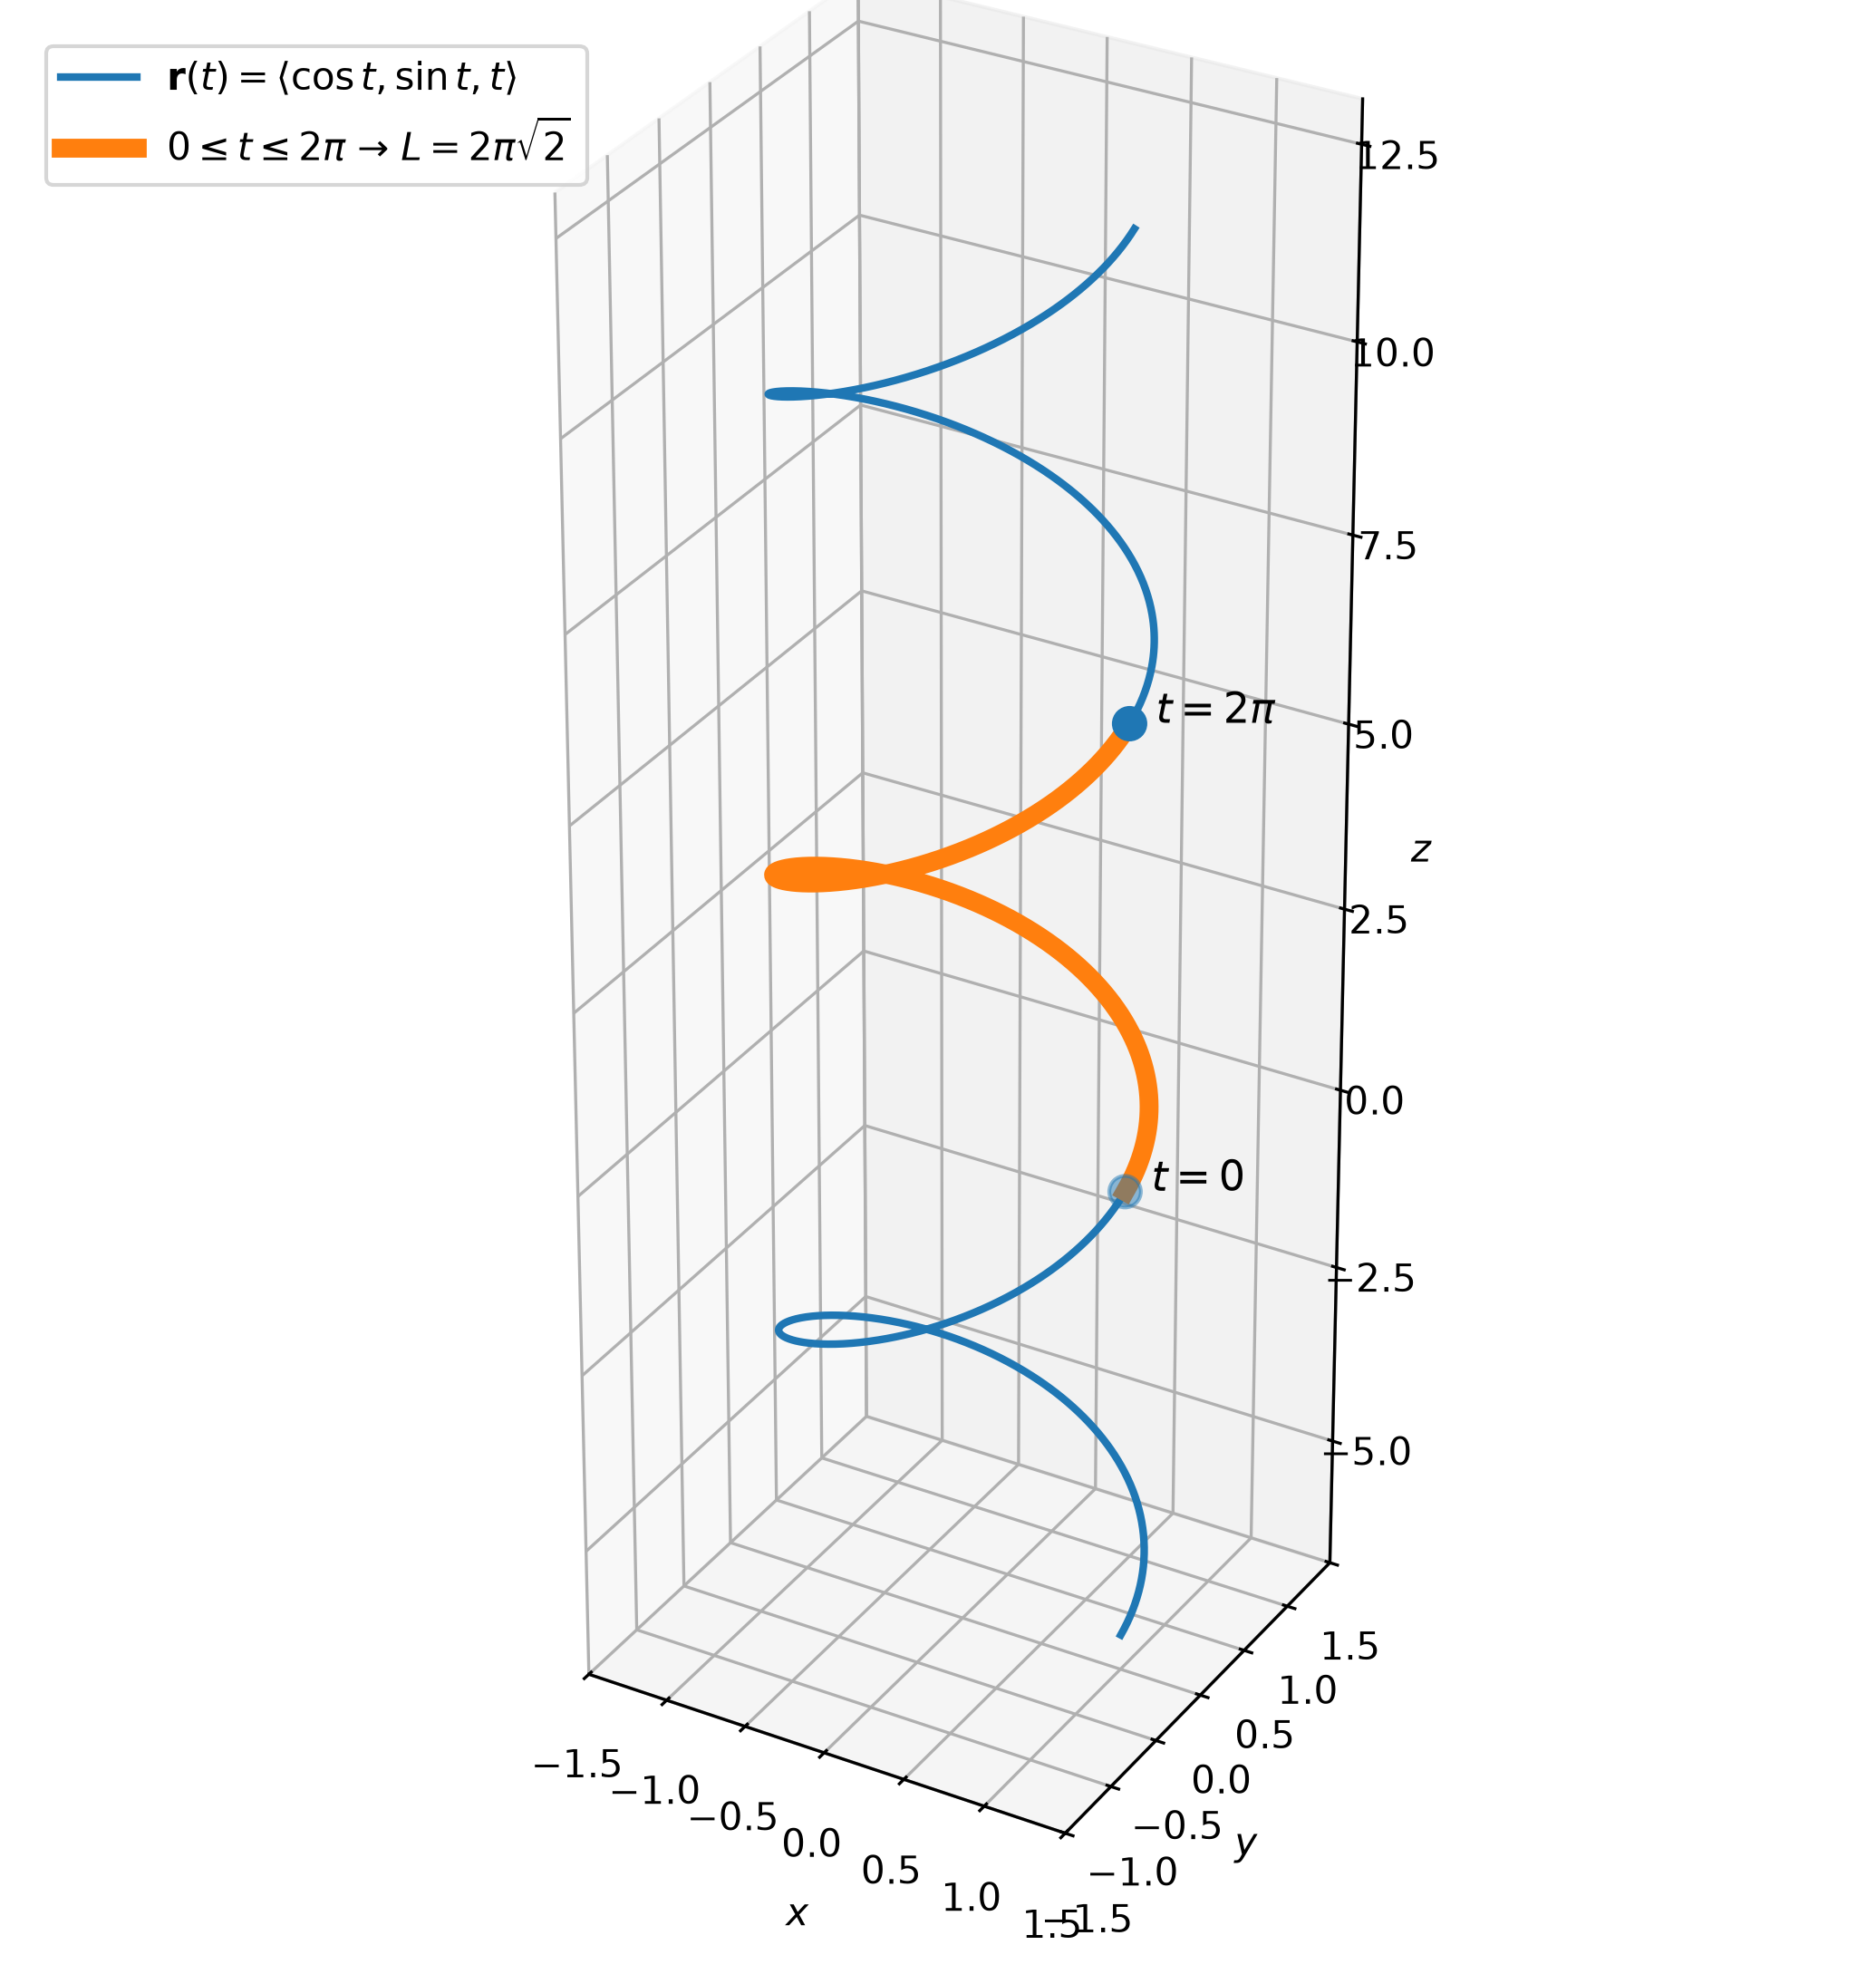
\includegraphics[width=0.5\textwidth]{./code/comprimento_de_arco.png}
    \caption{Hélice $\mathbf{r}(t)=\langle\cos t,\sin t,t\rangle$, com o intervalo
    $0\leq t\leq2\pi$ destacado.}
    \label{fig:comprimento-de-arco}
  \end{figure}
}

\question{
	Dada a curva

	\[
		\mathbf{r}(t)
		=
		\cos t\,\mathbf{i}
		+
		\sin t\,\mathbf{j}
		+
		t\,\mathbf{k},
	\]

	que tem como ponto de referência

	\[
		\mathbf{r}(0)=(1,0,0)
	\]

	e a mesma orientação que a hélice dada,
}

\subquestion{
	Determine a parametrização por comprimento de arco da hélice circular.
}

\answers{
	Para obter a parametrização por comprimento de arco, começamos
	calculando a derivada de $\mathbf{r}(t)$:

	\[
		\mathbf{r}'(t)
		=
		-\sin t\,\mathbf{i}
		+
		\cos t\,\mathbf{j}
		+
		\mathbf{k}.
	\]

	A velocidade escalar é

	\[
		\left\|\mathbf{r}'(t)\right\|
		=
		\sqrt{
			(-\sin t)^2
			+(\cos t)^2
			+1^2
		}.
	\]

	Usando a identidade

	\[
		\sin^2t+\cos^2t=1,
	\]

	obtemos

	\[
		\left\|\mathbf{r}'(t)\right\|
		=
		\sqrt{2}.
	\]

	Se $s$ representa o comprimento de arco medido a partir do ponto
	de referência $t=0$, então

	\[
		s
		=
		\int_0^t
		\left\|\mathbf{r}'(u)\right\|\,du.
	\]

	Como $\left\|\mathbf{r}'(u)\right\|=\sqrt{2}$,

	\[
		s
		=
		\int_0^t\sqrt{2}\,du
		=
		\sqrt{2}\,t.
	\]

	Logo,

	\[
		t=\frac{s}{\sqrt{2}}.
	\]

	Substituindo esse resultado na função vetorial original,

	\[
		\mathbf{r}(s)
		=
		\cos\left(\frac{s}{\sqrt{2}}\right)\mathbf{i}
		+
		\sin\left(\frac{s}{\sqrt{2}}\right)\mathbf{j}
		+
		\frac{s}{\sqrt{2}}\mathbf{k}.
	\]

	Portanto, a parametrização por comprimento de arco é

	\[
		\boxed{
		\mathbf{r}(s)
		=
		\left\langle
			\cos\left(\frac{s}{\sqrt{2}}\right),
			\sin\left(\frac{s}{\sqrt{2}}\right),
			\frac{s}{\sqrt{2}}
		\right\rangle
		}.
	\]

	Além disso,

	\[
		\left\|\mathbf{r}'(s)\right\|=1,
	]

	confirmando que $s$ é de fato o comprimento de arco.
}

\subquestion{
	Um besouro caminha pelo tronco de uma árvore seguindo uma trajetória
	$\mathbf{r}$. O besouro inicia no ponto de referência $(1,0,0)$ e sobe
	pela hélice por uma distância de $10$ unidades. Quais são as
	coordenadas finais do besouro?
}

\answers{
	Como $s$ representa o comprimento de arco medido a partir do ponto
	de referência, o besouro percorre

	\[
		s=10.
	\]

	Usando a parametrização por comprimento de arco,

	\[
		\mathbf{r}(s)
		=
		\left\langle
			\cos\left(\frac{s}{\sqrt{2}}\right),
			\sin\left(\frac{s}{\sqrt{2}}\right),
			\frac{s}{\sqrt{2}}
		\right\rangle,
	\]

	substituímos $s=10$:

	\[
		\mathbf{r}(10)
		=
		\left\langle
			\cos\left(\frac{10}{\sqrt{2}}\right),
			\sin\left(\frac{10}{\sqrt{2}}\right),
			\frac{10}{\sqrt{2}}
		\right\rangle.
	\]

	Como

	\[
		\frac{10}{\sqrt{2}}
		=
		5\sqrt{2},
	\]

	as coordenadas finais são

	\[
		\boxed{
		\left(
			\cos(5\sqrt{2}),
			\sin(5\sqrt{2}),
			5\sqrt{2}
		\right)
		}.
	\]

	Numericamente,

	\[
		\boxed{
		\left(
			0.7055,
			0.7087,
			7.0711
		\right)
		}.
	\]
}

\question{
	Determine a parametrização por comprimento de arco da reta

	\[
		x=2t+1,
		\qquad
		y=3t-2,
	\]

	que tem a mesma orientação que a reta dada e usa $(1,-2)$ como ponto
	de referência.
}

\answer{
	A reta pode ser representada pela função vetorial

	\[
		\mathbf{r}(t)
		=
		\left\langle
			2t+1,3t-2
		\right\rangle.
	\]

	O ponto de referência $(1,-2)$ corresponde a $t=0$, pois

	\[
		\mathbf{r}(0)
		=
		\left\langle
			1,-2
		\right\rangle.
	\]

	Calculando a derivada,

	\[
		\mathbf{r}'(t)
		=
		\left\langle
			2,3
		\right\rangle.
	\]

	A velocidade escalar da curva é

	\[
		\left\|\mathbf{r}'(t)\right\|
		=
		\sqrt{2^2+3^2}
		=
		\sqrt{13}.
	\]

	Se $s$ representa o comprimento de arco medido a partir do ponto de
	referência, então

	\[
		s
		=
		\int_0^t
		\left\|\mathbf{r}'(u)\right\|\,du
		=
		\int_0^t\sqrt{13}\,du.
	\]

	Logo,

	\[
		s=\sqrt{13}\,t,
	\]

	e, portanto,

	\[
		t=\frac{s}{\sqrt{13}}.
	\]

	Substituindo na função vetorial original,

	\[
		\mathbf{r}(s)
		=
		\left\langle
			2\frac{s}{\sqrt{13}}+1,
			3\frac{s}{\sqrt{13}}-2
		\right\rangle.
	\]

	Assim, a parametrização por comprimento de arco é

	\[
		\boxed{
		\mathbf{r}(s)
		=
		\left\langle
			1+\frac{2}{\sqrt{13}}s,
			-2+\frac{3}{\sqrt{13}}s
		\right\rangle
		}.
	\]

	Como

	\[
		\mathbf{r}'(s)
		=
		\left\langle
			\frac{2}{\sqrt{13}},
			\frac{3}{\sqrt{13}}
		\right\rangle
	\]

	e

	\[
		\left\|\mathbf{r}'(s)\right\|
		=
		1,
	\]

	confirmamos que $s$ é o comprimento de arco. Além disso, o vetor
	tangente mantém a mesma orientação da reta original.
}

\section*{Vetores Tangente, Normal e Binormal Unitários}

\definition{Vetor Tangente Unitário}{
	Seja $C$ o gráfico de uma função vetorial lisa $\mathbf{r}(t)$ no espaço
	bidimensional ou tridimensional. Se $\mathbf{r}'(t)\neq\mathbf{0}$, então
	$\mathbf{r}'(t)$ é tangente a $C$ e aponta no sentido do parâmetro
	crescente.

	O \textbf{vetor tangente unitário} é obtido normalizando
	$\mathbf{r}'(t)$:

	\[
		\boxed{
		\mathbf{T}(t)
		=
		\frac{\mathbf{r}'(t)}
		{\left\|\mathbf{r}'(t)\right\|}
		}.
	\]

	Assim, $\mathbf{T}(t)$ é um vetor unitário tangente à curva e aponta no
	sentido do parâmetro crescente.
}

\question{
	Encontre o vetor tangente unitário ao gráfico de

	\[
		\mathbf{r}(t)
		=
		t^2\mathbf{i}+t^3\mathbf{j}
	\]

	no ponto em que $t=2$.
}

\answer{
	Primeiramente, calculamos a derivada:

	\[
		\mathbf{r}'(t)
		=
		2t\mathbf{i}+3t^2\mathbf{j}.
	\]

	Em $t=2$,

	\[
		\mathbf{r}'(2)
		=
		4\mathbf{i}+12\mathbf{j}.
	\]

	A norma desse vetor é

	\[
		\left\|\mathbf{r}'(2)\right\|
		=
		\sqrt{4^2+12^2}
		=
		\sqrt{160}
		=
		4\sqrt{10}.
	\]

	Portanto,

	\[
		\mathbf{T}(2)
		=
		\frac{4\mathbf{i}+12\mathbf{j}}
		{4\sqrt{10}}
		=
		\boxed{
		\frac{1}{\sqrt{10}}\mathbf{i}
		+
		\frac{3}{\sqrt{10}}\mathbf{j}
		}.
	}
}

\definition{Vetor Normal Unitário}{
	Seja $\mathbf{T}(t)$ o vetor tangente unitário de uma curva. Como
	$\|\mathbf{T}(t)\|=1$, o vetor $\mathbf{T}'(t)$ é ortogonal a
	$\mathbf{T}(t)$.

	Quando

	\[
		\mathbf{T}'(t)\neq\mathbf{0},
	\]

	o \textbf{vetor normal unitário principal} é definido por

	\[
		\boxed{
		\mathbf{N}(t)
		=
		\frac{\mathbf{T}'(t)}
		{\left\|\mathbf{T}'(t)\right\|}
		}.
	\]

	O vetor $\mathbf{N}(t)$ é perpendicular à reta tangente e aponta na
	mesma direção e sentido que $\mathbf{T}'(t)$.

	O vetor normal unitário somente está definido nos pontos em que

	\[
		\mathbf{T}'(t)\neq\mathbf{0}.
	\]

	Em particular, retas possuem vetor tangente unitário constante e,
	portanto, não possuem vetor normal unitário principal definido dessa
	maneira.
}

\definition{Normal Unitário para Dentro}{
	Em uma curva paramétrica não linear no espaço bidimensional, o vetor
	normal unitário principal aponta para o lado côncavo da curva.

	Por essa razão, em curvas planas, $\mathbf{N}(t)$ é também chamado de
	\textbf{normal unitário para dentro}.
}

\question{
	Obtenha $\mathbf{T}(t)$ e $\mathbf{N}(t)$ para a hélice circular

	\[
		\begin{cases}
			x=a\cos t,\\
			y=a\sin t,\\
			z=ct,
		\end{cases}
		\qquad a>0.
	}
	
\answer{
	A função vetorial que representa a hélice é

	\[
		\mathbf{r}(t)
		=
		a\cos t\,\mathbf{i}
		+
		a\sin t\,\mathbf{j}
		+
		ct\,\mathbf{k}.
	\]

	Derivando,

	\[
		\mathbf{r}'(t)
		=
		-a\sin t\,\mathbf{i}
		+
		a\cos t\,\mathbf{j}
		+
		c\mathbf{k}.
	\]

	Sua norma é

	\[
		\left\|\mathbf{r}'(t)\right\|
		=
		\sqrt{
			a^2\sin^2t+a^2\cos^2t+c^2
		}
		=
		\sqrt{a^2+c^2}.
	\]

	Portanto,

	\[
		\boxed{
		\mathbf{T}(t)
		=
		\frac{
			-a\sin t\,\mathbf{i}
			+a\cos t\,\mathbf{j}
			+c\mathbf{k}
		}
		{\sqrt{a^2+c^2}}
		}.
	\]

	Como $a$ e $c$ são constantes,

	\[
		\mathbf{T}'(t)
		=
		\frac{
			-a\cos t\,\mathbf{i}
			-a\sin t\,\mathbf{j}
		}
		{\sqrt{a^2+c^2}}.
	\]

	Sua norma é

	\[
		\left\|\mathbf{T}'(t)\right\|
		=
		\frac{a}{\sqrt{a^2+c^2}}.
	\]

	Assim,

	\[
		\boxed{
		\mathbf{N}(t)
		=
		-\cos t\,\mathbf{i}
		-\sin t\,\mathbf{j}
		}.
	\]

	Observe que o componente na direção $\mathbf{k}$ é zero. Portanto,
	$\mathbf{N}(t)$ está sempre em um plano horizontal e aponta em direção
	ao eixo $z$.
}

\definition{Normal Unitário em uma Curva Plana}{
	Considere uma curva no espaço bidimensional e seja $\phi(t)$ o ângulo
	entre o eixo $x$ positivo e o vetor tangente unitário $\mathbf{T}(t)$.

	Podemos escrever

	\[
		\mathbf{T}(t)
		=
		\cos\phi(t)\mathbf{i}
		+
		\sin\phi(t)\mathbf{j}.
	\]

	Se $\mathbf{n}(t)$ for obtido girando $\mathbf{T}(t)$ no sentido
	anti-horário por um ângulo de $\pi/2$, então

	\[
		\mathbf{n}(t)
		=
		-\sin\phi(t)\mathbf{i}
		+
		\cos\phi(t)\mathbf{j}.
	\]

	Derivando $\mathbf{T}(t)$,

	\[
		\mathbf{T}'(t)
		=
		\frac{d\phi}{dt}
		\mathbf{n}(t).
	\]

	Assim, quando $\phi(t)$ é crescente, $\mathbf{T}'(t)$ possui a mesma
	direção e sentido que $\mathbf{n}(t)$. Quando $\phi(t)$ é decrescente,
	$\mathbf{T}'(t)$ possui sentido oposto.

	Em ambos os casos, após a normalização de $\mathbf{T}'(t)$, o vetor
	normal unitário principal aponta para o lado côncavo da curva.
}

\definition{Vetor Tangente Unitário Parametrizado pelo Comprimento de Arco}{
	Se $\mathbf{r}(s)$ é uma parametrização de uma curva pelo comprimento de
	arco, então

	\[
		\left\|\mathbf{r}'(s)\right\|=1.
	\]

	Consequentemente, o vetor tangente unitário assume a forma simplificada

	\[
		\boxed{
		\mathbf{T}(s)=\mathbf{r}'(s)
		}.
	\]
}

\definition{Vetor Normal Unitário Parametrizado pelo Comprimento de Arco}{
	Se $\mathbf{r}(s)$ é parametrizada pelo comprimento de arco, então

	\[
		\mathbf{T}(s)=\mathbf{r}'(s).
	\]

	Portanto,

	\[
		\mathbf{T}'(s)=\mathbf{r}''(s).
	\]

	Assim, o vetor normal unitário pode ser calculado diretamente por

	\[
		\boxed{
		\mathbf{N}(s)
		=
		\frac{\mathbf{r}''(s)}
		{\left\|\mathbf{r}''(s)\right\|}
		},
	\]

	desde que $\mathbf{r}''(s)\neq\mathbf{0}$.
}

\question{
	O círculo de raio $a$, orientado no sentido anti-horário e centrado na
	origem, é representado por

	\[
		\mathbf{r}(t)
		=
		a\cos t\,\mathbf{i}
		+
		a\sin t\,\mathbf{j},
		\qquad
		0\leq t\leq2\pi.
		\]

	Parametrize o círculo pelo comprimento de arco e encontre
	$\mathbf{T}(s)$ e $\mathbf{N}(s)$.
}

\answer{
	No círculo de raio $a$, o comprimento do arco correspondente ao ângulo
	$t$ é

	\[
		s=at.
	\]

	Portanto,

	\[
		t=\frac{s}{a}.
	\]

	Substituindo na parametrização original,

	\[
		\mathbf{r}(s)
		=
		a\cos\left(\frac{s}{a}\right)\mathbf{i}
		+
		a\sin\left(\frac{s}{a}\right)\mathbf{j},
		\qquad
		0\leq s\leq2\pi a.
	\]

	Como a curva está parametrizada pelo comprimento de arco,

	\[
		\mathbf{T}(s)=\mathbf{r}'(s).
	\]

	Assim,

	\[
		\mathbf{T}(s)
		=
		-\sin\left(\frac{s}{a}\right)\mathbf{i}
		+
		\cos\left(\frac{s}{a}\right)\mathbf{j}.
	\]

	Derivando novamente,

	\[
		\mathbf{T}'(s)
		=
		-\frac{1}{a}
		\cos\left(\frac{s}{a}\right)\mathbf{i}
		-
		\frac{1}{a}
		\sin\left(\frac{s}{a}\right)\mathbf{j}.
	\]

	Como

	\[
		\left\|\mathbf{T}'(s)\right\|
		=
		\frac{1}{a},
	\]

	obtemos

	\[
		\boxed{
		\mathbf{N}(s)
		=
		-\cos\left(\frac{s}{a}\right)\mathbf{i}
		-
		\sin\left(\frac{s}{a}\right)\mathbf{j}
		}.
	\]

	Portanto,

	\[
		\boxed{
		\mathbf{T}(s)
		=
		-\sin\left(\frac{s}{a}\right)\mathbf{i}
		+
		\cos\left(\frac{s}{a}\right)\mathbf{j}
		}
	\]

	e

	\[
		\boxed{
		\mathbf{N}(s)
		=
		-\cos\left(\frac{s}{a}\right)\mathbf{i}
		-
		\sin\left(\frac{s}{a}\right)\mathbf{j}
		}.
	\]

	O vetor $\mathbf{N}(s)$ aponta para o centro do círculo, como esperado
	geometricamente.
}

\definition{Vetor Binormal}{
	Se $C$ for o gráfico de uma função vetorial $\mathbf{r}(t)$ no espaço
	tridimensional, o \textbf{vetor binormal} é definido por

	\[
		\boxed{
		\mathbf{B}(t)
		=
		\mathbf{T}(t)\times\mathbf{N}(t)
		}.
	\]

	Como $\mathbf{T}(t)$ e $\mathbf{N}(t)$ são vetores unitários
	ortogonais,

	\[
		\left\|\mathbf{B}(t)\right\|=1.
	\]

	Além disso, $\mathbf{B}(t)$ é ortogonal tanto a $\mathbf{T}(t)$ quanto
	a $\mathbf{N}(t)$.

	O sentido de $\mathbf{B}(t)$ é determinado pela regra da mão direita.
}

\definition{Triedro de Frenet}{
	Os vetores

	\[
		\mathbf{T}(t),\qquad
		\mathbf{N}(t),\qquad
		\mathbf{B}(t)
	\]

	formam três vetores unitários mutuamente ortogonais e determinam um
	sistema de coordenadas móvel associado à curva, denominado
	\textbf{triedro de Frenet} ou \textbf{triedro TNB}.

	Esses vetores satisfazem as relações

	\[
		\boxed{
		\mathbf{B}
		=
		\mathbf{T}\times\mathbf{N}
		},
	\]

	\[
		\boxed{
		\mathbf{N}
		=
		\mathbf{B}\times\mathbf{T}
		},
	\]

	e

	\[
		\boxed{
		\mathbf{T}
		=
		\mathbf{N}\times\mathbf{B}
		}.
	\]

	Os três vetores determinam três planos mutuamente perpendiculares:

	\begin{itemize}
		\item o plano $TB$, chamado \textbf{plano retificante};
		\item o plano $TN$, chamado \textbf{plano osculador};
		\item o plano $NB$, chamado \textbf{plano normal}.
	\end{itemize}

	A diferença entre o sistema de coordenadas fixo
	$(\mathbf{i},\mathbf{j},\mathbf{k})$ e o triedro de Frenet é que o primeiro
	permanece fixo, enquanto o triedro TNB se desloca e gira ao longo da
	curva.
}

\definition{Vetor Binormal em Termos da Função Vetorial}{
	O vetor binormal também pode ser calculado diretamente a partir da
	função vetorial $\mathbf{r}(t)$ por

	\[
	\boxed{
	\mathbf{B}(t)
	=
	\frac{
		\mathbf{r}'(t)\times\mathbf{r}''(t)
	}{
		\left\|
			mathbf{r}'(t)\times\mathbf{r}''(t)
		\right\|
	}
	}.
	\]

	Quando a curva está parametrizada pelo comprimento de arco, temos

	\[
		\mathbf{r}'(s)=\mathbf{T}(s)
	\]

	e

	\[
		\mathbf{r}''(s)=\mathbf{T}'(s).
	\]

	Consequentemente,

	\[
	\boxed{
	\mathbf{B}(s)
	=
	\frac{
		\mathbf{r}'(s)\times\mathbf{r}''(s)
	}{
		\left\|
			\mathbf{r}'(s)\times\mathbf{r}''(s)
		\right\|
	}
	}.
\]
}

\subquestion{
	Qual é a relação geométrica entre os vetores $\mathbf{T}$,
	$\mathbf{N}$ e $\mathbf{B}$?
}

\answer{
	Os três vetores são unitários e mutuamente ortogonais:

	\[
		\mathbf{T}\cdot\mathbf{N}=0,
		\qquad
		\mathbf{T}\cdot\mathbf{B}=0,
		\qquad
		\mathbf{N}\cdot\mathbf{B}=0.
	\]

	Além disso,

	\[
		\mathbf{B}=\mathbf{T}\times\mathbf{N},
	\]

	de modo que $\mathbf{T}$, $\mathbf{N}$ e $\mathbf{B}$ formam um sistema
	de coordenadas orientado pela regra da mão direita.

	O vetor $\mathbf{T}$ indica a direção do movimento ao longo da curva,
	$\mathbf{N}$ indica a direção na qual a curva está se desviando e
	$\mathbf{B}$ indica a direção perpendicular ao plano determinado por
	$\mathbf{T}$ e $\mathbf{N}$.
}

\section*{Curvatura}

\definition{Curvatura}{
	Seja $C$ uma curva lisa no espaço bidimensional ou tridimensional
	parametrizada pelo comprimento de arco $s$. A \textbf{curvatura} de $C$,
	denotada por $\kappa=\kappa(s)$, é definida por

	\[
		\boxed{
		\kappa(s)
		=
		\left\|
			\frac{d\mathbf{T}}{ds}
		\right\|
		}.
	\]

	A curvatura mede a intensidade com que a curva se encurva. Como
	$\mathbf{T}(s)$ é um vetor unitário, sua norma permanece constante e
	somente sua direção varia. Portanto, quanto mais rapidamente a direção
	de $\mathbf{T}$ variar em relação ao comprimento de arco, maior será a
	curvatura.

	Para uma reta, a direção de $\mathbf{T}$ permanece constante e,
	consequentemente,

	\[
		\boxed{\kappa=0}.
	\]

	Para um círculo de raio $a$, a curvatura é constante e vale

	\[
		\boxed{\kappa=\frac{1}{a}}.
	\]
}

\question{
	Determine a curvatura de um círculo de raio $a$ centrado na origem.
}

\answer{
	Parametrizando o círculo pelo comprimento de arco, temos

	\[
		\mathbf{r}(s)
		=
		a\cos\left(\frac{s}{a}\right)\mathbf{i}
		+
		a\sin\left(\frac{s}{a}\right)\mathbf{j}.
	\]

	O vetor tangente unitário é

	\[
		\mathbf{T}(s)
		=
		-\sin\left(\frac{s}{a}\right)\mathbf{i}
		+
		\cos\left(\frac{s}{a}\right)\mathbf{j}.
	\]

	Derivando em relação a $s$,

	\[
		\frac{d\mathbf{T}}{ds}
		=
		-\frac{1}{a}
		\cos\left(\frac{s}{a}\right)\mathbf{i}
		-
		\frac{1}{a}
		\sin\left(\frac{s}{a}\right)\mathbf{j}.
	\]

	Logo,

	\[
		\kappa(s)
		=
		\left\|
			\frac{d\mathbf{T}}{ds}
		\right\|
		=
		\frac{1}{a}
		\sqrt{
			\cos^2\left(\frac{s}{a}\right)
			+
			\sin^2\left(\frac{s}{a}\right)
		}.
	\]

	Como $\sin^2u+\cos^2u=1$,

	\[
		\boxed{
		\kappa=\frac{1}{a}
		}.
	\]

	Portanto, a curvatura do círculo é constante.
}

\question{
	Mostre que uma reta possui curvatura igual a zero.
}

\answer{
	Uma reta pode ser parametrizada pelo comprimento de arco na forma

	\[
		\mathbf{r}(s)
		=
		\mathbf{r}_0+s\mathbf{u},
	\]

	onde $\mathbf{r}_0$ é um vetor constante e $\mathbf{u}$ é um vetor
	unitário constante paralelo à reta.

	Derivando,

	\[
		\mathbf{r}'(s)=\mathbf{u}.
	\]

	Assim, o vetor tangente unitário é constante:

	\[
		\mathbf{T}(s)=\mathbf{u}.
	\]

	Portanto,

	\[
		\frac{d\mathbf{T}}{ds}
		=
		\mathbf{0}.
	\]

	Consequentemente,

	\[
		\boxed{
		\kappa(s)
		=
		\left\|
			\frac{d\mathbf{T}}{ds}
		\right\|
		=
		0
		}.
	\]

	Isso é consistente com a interpretação geométrica de que uma reta não
	possui encurvamento.
}

\definition{Fórmula da Curvatura em Termos de um Parâmetro Qualquer}{
	Se $\mathbf{r}(t)$ for uma função vetorial lisa no espaço bidimensional
	ou tridimensional, a curvatura pode ser calculada sem que a curva esteja
	parametrizada pelo comprimento de arco.

	Uma das formas é

	\[
		\boxed{
		\kappa(t)
		=
		\frac{
			\left\|\mathbf{T}'(t)\right\|
		}{
			\left\|\mathbf{r}'(t)\right\|
		}
		}.
	\]

	Essa fórmula é útil quando o vetor tangente unitário
	$\mathbf{T}(t)$ é conhecido ou pode ser obtido facilmente.

	Existe também uma fórmula que depende somente de $\mathbf{r}(t)$ e de
	suas derivadas:

	\[
		\boxed{
		\kappa(t)
		=
		\frac{
			\left\|
				\mathbf{r}'(t)\times\mathbf{r}''(t)
			\right\|
		}{
			\left\|\mathbf{r}'(t)\right\|^3
		}
		}.
	\]

	Para curvas no espaço bidimensional, interpretamos

	\[
		\mathbf{r}(t)
		=
		x(t)\mathbf{i}+y(t)\mathbf{j}
	\]

	como uma curva tridimensional escrevendo

	\[
		\mathbf{r}(t)
		=
		x(t)\mathbf{i}
		+
		y(t)\mathbf{j}
		+
		0\mathbf{k}.
	\]

	Assim, o produto vetorial pode ser calculado normalmente.
}

\question{
	Determine a curvatura da hélice circular

	\[
		\mathbf{r}(t)
		=
		a\cos t\,\mathbf{i}
		+
		a\sin t\,\mathbf{j}
		+
		ct\,\mathbf{k},
	\]

	onde $a>0$.
}

\answer{
	Calculamos inicialmente as derivadas da função vetorial:

	\[
		\mathbf{r}'(t)
		=
		-a\sin t\,\mathbf{i}
		+
		a\cos t\,\mathbf{j}
		+
		c\mathbf{k},
	\]

	e

	\[
		\mathbf{r}''(t)
		=
		-a\cos t\,\mathbf{i}
		-
		a\sin t\,\mathbf{j}.
	\]

	A norma de $\mathbf{r}'(t)$ é

	\[
		\left\|\mathbf{r}'(t)\right\|
		=
		\sqrt{
			a^2\sin^2t+a^2\cos^2t+c^2
		}
		=
		\sqrt{a^2+c^2}.
	\]

	Agora calculamos o produto vetorial:

	\[
		\mathbf{r}'(t)\times\mathbf{r}''(t)
		=
		\begin{vmatrix}
			\mathbf{i}&\mathbf{j}&\mathbf{k}\\
			-a\sin t&a\cos t&c\\
			-a\cos t&-a\sin t&0
		\end{vmatrix}.
	\]

	Desenvolvendo o determinante,

	\[
		\mathbf{r}'(t)\times\mathbf{r}''(t)
		=
		\left\langle
			ac\sin t,
			-ac\cos t,
			a^2
		\right\rangle.
	\]

	Sua norma é

	\[
		\left\|
			\mathbf{r}'(t)\times\mathbf{r}''(t)
		\right\|
		=
		\sqrt{
			a^2c^2\sin^2t
			+
			a^2c^2\cos^2t
			+
			a^4
		}.
	\]

	Portanto,

	\[
		\left\|
			\mathbf{r}'(t)\times\mathbf{r}''(t)
		\right\|
		=
		a\sqrt{a^2+c^2}.
	\]

	Aplicando a fórmula da curvatura,

	\[
		\kappa(t)
		=
		\frac{
			a\sqrt{a^2+c^2}
		}{
			\left(\sqrt{a^2+c^2}\right)^3
		}.
	\]

	Logo,

	\[
		\boxed{
		\kappa(t)
		=
		\frac{a}{a^2+c^2}
		}.
	\]

	Observe que a curvatura não depende de $t$. Portanto, a hélice possui
	curvatura constante.
}

\question{
	Considere a elipse

	\[
		\mathbf{r}(t)
		=
		2\cos t\,\mathbf{i}
		+
		3\sin t\,\mathbf{j},
		\qquad
		0\leq t\leq2\pi.
	\]

	Determine a curvatura nos extremos dos eixos maior e menor.
}

\answer{
	Para aplicar a fórmula da curvatura, escrevemos a curva no espaço
	tridimensional como

	\[
		\mathbf{r}(t)
		=
		2\cos t\,\mathbf{i}
		+
		3\sin t\,\mathbf{j}
		+
		0\mathbf{k}.
	\]

	Temos

	\[
		\mathbf{r}'(t)
		=
		-2\sin t\,\mathbf{i}
		+
		3\cos t\,\mathbf{j},
	\]

	e

	\[
		\mathbf{r}''(t)
		=
		-2\cos t\,\mathbf{i}
		-
		3\sin t\,\mathbf{j}.
	\]

	O produto vetorial é

	\[
		\mathbf{r}'(t)\times\mathbf{r}''(t)
		=
		6\mathbf{k}.
	\]

	Portanto,

	\[
		\left\|
			\mathbf{r}'(t)\times\mathbf{r}''(t)
		\right\|
		=
		6.
	\]

	Além disso,

	\[
		\left\|\mathbf{r}'(t)\right\|
		=
		\sqrt{
			4\sin^2t+9\cos^2t
		}.
	\]

	Logo,

	\[
		\boxed{
		\kappa(t)
		=
		\frac{6}
		{
			\left(
				4\sin^2t+9\cos^2t
			\right)^{3/2}
		}
		}.
	\]

	As extremidades do eixo menor são

	\[
		(2,0)
		\qquad\text{e}\qquad
		(-2,0),
	\]

	que correspondem a $t=0$ e $t=\pi$.

	Em $t=0$,

	\[
		\kappa(0)
		=
		\frac{6}{9^{3/2}}
		=
		\frac{6}{27}
		=
		\boxed{\frac{2}{9}}.
	\]

	Como $\kappa(\pi)=\kappa(0)$,

	\[
		\boxed{
		\kappa(0)=\kappa(\pi)=\frac{2}{9}
		}.
	\]

	As extremidades do eixo maior são

	\[
		(0,3)
		\qquad\text{e}\qquad
		(0,-3),
	\]

	que correspondem a $t=\frac{\pi}{2}$ e $t=\frac{3\pi}{2}$.

	Em $t=\frac{\pi}{2}$,

	\[
		\kappa\left(\frac{\pi}{2}\right)
		=
		\frac{6}{4^{3/2}}
		=
		\frac{6}{8}
		=
		\boxed{\frac{3}{4}}.
	\]

	Assim,

	\[
		\boxed{
		\kappa\left(\frac{\pi}{2}\right)
		=
		\kappa\left(\frac{3\pi}{2}\right)
		=
		\frac{3}{4}
		}.
	\]

	Portanto, a curvatura é maior nas extremidades do eixo maior:

	\[
		\frac{3}{4}>\frac{2}{9}.
	\]

	Isso significa que a elipse se encurva mais intensamente nas
	extremidades do seu eixo maior.
}

\definition{Raio de Curvatura}{
	Se uma curva possui curvatura $\kappa$ em um ponto $P$, define-se o
	\textbf{raio de curvatura} $\rho$ nesse ponto por

	\[
		\boxed{
		\rho=\frac{1}{\kappa}
		}.
	\]

	No espaço bidimensional, o círculo de raio $\rho$ que possui a mesma
	tangente que a curva em $P$ e cujo centro está no lado côncavo da curva
	é chamado de \textbf{círculo de curvatura} ou \textbf{círculo osculador}.

	O círculo osculador possui a mesma curvatura que a curva no ponto $P$ e,
	portanto, fornece uma aproximação circular local da curva.

	O centro desse círculo é chamado de \textbf{centro de curvatura}.
}

\question{
	Determine o raio de curvatura da elipse

	\[
		\mathbf{r}(t)
		=
		2\cos t\,\mathbf{i}
		+
		3\sin t\,\mathbf{j}
	\]

	nas extremidades dos eixos maior e menor.
}

\answer{
	Nas extremidades do eixo menor, temos

	\[
		\kappa=\frac{2}{9}.
	\]

	Portanto,

	\[
		\rho
		=
		\frac{1}{\kappa}
		=
		\frac{1}{2/9}
		=
		\boxed{\frac{9}{2}}.
	\]

	Nas extremidades do eixo maior,

	\[
		\kappa=\frac{3}{4}.
	\]

	Assim,

	\[
		\rho
		=
		\frac{1}{3/4}
		=
		\boxed{\frac{4}{3}}.
	\]

	Portanto,

	\[
		\boxed{
		\rho_{\text{eixo menor}}=\frac{9}{2}
		}
	\]

	e

	\[
		\boxed{
		\rho_{\text{eixo maior}}=\frac{4}{3}
		}.
	\]

	Como maior curvatura corresponde a menor raio de curvatura, o círculo
	osculador é menor nas extremidades do eixo maior.
}

\definition{Interpretação da Curvatura no Espaço Bidimensional}{
	Considere uma curva plana e seja $\phi$ o ângulo medido no sentido
	anti-horário a partir do eixo $x$ positivo até o vetor tangente unitário
	$\mathbf{T}$.

	Podemos escrever

	\[
		\mathbf{T}
		=
		\cos\phi\,\mathbf{i}
		+
		\sin\phi\,\mathbf{j}.
	\]

	Como $s$ é o comprimento de arco,

	\[
		\frac{d\mathbf{T}}{ds}
		=
		\frac{d\phi}{ds}
		\left(
			-\sin\phi\,\mathbf{i}
			+
			\cos\phi\,\mathbf{j}
		\right).
	\]

	Tomando a norma,

	\[
		\boxed{
		\kappa
		=
		\left|
			\frac{d\phi}{ds}
		\right|
		}.
	\]

	Assim, a curvatura pode ser interpretada como a magnitude da taxa de
	variação do ângulo do vetor tangente unitário em relação ao comprimento
	de arco.

	Quanto maior for $\kappa$, mais rapidamente a direção da tangente varia
	ao longo da curva.

	Para uma reta, $\phi$ é constante. Portanto,

	\[
		\frac{d\phi}{ds}=0
	\]

	e, consequentemente,

	\[
		\kappa=0.
	\]
}

\question{
	Qual é a relação entre curvatura e a variação da direção do vetor
	tangente unitário em uma curva plana?
}

\answer{
	A curvatura é dada por

	\[
		\boxed{
		\kappa
		=
		\left|
			\frac{d\phi}{ds}
		\right|
		},
	\]

	onde $\phi$ é o ângulo que o vetor tangente unitário $\mathbf{T}$ forma
	com o eixo $x$ positivo.

	Portanto, a curvatura mede a rapidez com que a direção de $\mathbf{T}$
	muda em relação ao comprimento de arco.

	Se $\kappa$ for grande, a direção da curva muda rapidamente. Se $\kappa$
	for pequena, a direção muda lentamente. Para uma reta,

	\[
		\boxed{\kappa=0},
	\]

	pois seu vetor tangente unitário possui direção constante.
}

\definition{Resumo das Fórmulas de Curvatura e do Triedro TNB}{
	Para uma curva lisa $\mathbf{r}(t)$, os vetores tangente, normal e
	binormal unitários são dados por

	\[
		\boxed{
		\mathbf{T}(t)
		=
		\frac{\mathbf{r}'(t)}
		{\left\|\mathbf{r}'(t)\right\|}
		},
	\]

	\[
		\boxed{
		\mathbf{N}(t)
		=
		\frac{\mathbf{T}'(t)}
		{\left\|\mathbf{T}'(t)\right\|}
		},
	\]

	e

	\[
		\boxed{
		\mathbf{B}(t)
		=
		\mathbf{T}(t)\times\mathbf{N}(t)
		}.
	\]

	A curvatura pode ser calculada por

	\[
		\boxed{
		\kappa(t)
		=
		\frac{
			\left\|\mathbf{T}'(t)\right\|
		}{
			\left\|\mathbf{r}'(t)\right\|
		}
		}
	\]

	ou, diretamente em termos de $\mathbf{r}(t)$,

	\[
		\boxed{
		\kappa(t)
		=
		\frac{
			\left\|
				\mathbf{r}'(t)\times\mathbf{r}''(t)
			\right\|
		}{
			\left\|\mathbf{r}'(t)\right\|^3
		}
		}.
	\]

	Quando a curva está parametrizada pelo comprimento de arco $s$,

	\[
		\boxed{
		\mathbf{T}(s)=\mathbf{r}'(s)
		}
	\]

	e

	\[
		\boxed{
		\mathbf{N}(s)
		=
		\frac{\mathbf{r}''(s)}
		{\left\|\mathbf{r}''(s)\right\|}
		}.
	\]

	Nesse caso,

	\[
		\boxed{
		\kappa(s)
		=
		\left\|\mathbf{r}''(s)\right\|
		}.
	\]

	Finalmente, o raio de curvatura é

	\[
		\boxed{
		\rho=\frac{1}{\kappa}
		}.
	\]
}
